\scanpage{210}
The system of groups \inserted{over $\mathbb{Q}$} (36, 37), equipped
with the homomorphism from
\[
\Pi \subset \mathcal{G} \subset M
\]
into \deleted{\unsure{$\mathcal{G}$}}
\[
(40)\qquad
\underline{\Pi}_{\mathbb{Q}}(\unsure{\mathbb{A}'_{\mathbb{Q}}})
\subset \underline{\mathcal{G}}_{\mathbb{Q}}(\mathbb{A}_{\mathbb{Q}})
\subset \underline{M}_{\mathbb{Q}}(\unsure{\mathbb{A}_{\mathbb{Q}}})
\]
\deleted{deduced} \inserted{induced} by
$M\longrightarrow \unsure{G}(\mathbb{A}_{\mathbb{Q}})$ (satisfying
conditions $1^\circ)$ to $4^\circ)$ above \deleted{\unsure{)}}, i.e.
of a ``Lie homomorphism'') will also be called
a ``\uline{Lie approximation}'' of the
Galois-Teichmüller system under consideration.

Consider a \deleted{germ of a }homomorphism
\[
(41)\qquad k_i^{\deleted{\unsure{\sharp}}}\quad T_0\longrightarrow\Pi_0
\]
\unsure{belonging|corresponding} to the L-structure of $\Pi$,
thus defines \inserted{by composition with
$\unsure{\Pi_0}\longrightarrow
\deleted{\unsure{\mathcal{G}}}\underline{\Pi}_{\deleted{\unsure{\mathbb{Q}}}}(\mathbb{Q})$}
a \deleted{germ of a }homomorphism
\[
(42)\qquad T_0\longrightarrow
\deleted{\unsure{\mathcal{G}}}\underline{\Pi}(\mathbb{Q}).
\]
\margin{\uline{N.B.} for fixed $i$,
$k_i$ is determined modulo
inner \unsure{automorphisms} of $\Pi_0$ \uuline{and}
modulo composition with
$n\,\mathrm{id}_{T_0}$, for $n\in\mathbb{N}^{*}$.
As for this last point, \unsure{there is}
\unsure{often} (\unsure{let us fix} $\Pi_0$) a
``best choice'', from which all \unsure{the others are}
deduced by composition with
$n\,\mathrm{id}_{T_0}$.}
We see \inserted{((21) page\,$747'$)} that this \deleted{germ of a} homomorphism
is quasi-unipotent, and that it therefore defines
a homomorphism of \deleted{\unsure{g}} group schemes
\margin{209}

\scanpage{211}
\mspage{753}
\[
(43)\qquad \underline{k}_i:
\underset{(\simeq G_{a\mathbb{Q}}\otimes_{\mathbb{Z}}T_0)}{\underline{T}_{0\mathbb{Q}}}
\longrightarrow \underline{\Pi}_{\mathbb{Q}}
\]
(not just a germ!)
which defines, by \deleted{composition} passage to
the $\mathbb{Q}$-rational points, the \uline{germ} of the homomorphism
(42). We thus find a finite set
(indexed by \inserted{the set} of germs of loop \uline{subgroups}
of $\Pi_0$, or of $\Pi$ which amounts \unsure{to the}
\unsure{same}) of outer homomorphisms (43) of group
schemes. I feel like calling the Lie appro-\deleted{\unsure{representation}}\inserted{ximation} \uline{nondegenerate} if
the preceding homomorphisms are all nontrivial,
hence are \uline{monomorphisms}.
\[
(44)\qquad \underline{k}_i:
\underline{T}_{0\mathbb{Q}}\simeq G_{a\mathbb{Q}}\otimes_{\mathbb{Z}}T_0
\lhook\joinrel\longrightarrow \underline{\Pi}_{\mathbb{Q}}.
\]

Suppose that $\underline{M}_{\mathbb{Q}}$ comes from
a group scheme (affine \unsure{and} of finite type)
$\underline{M}$ over $\mathbb{Z}$, such that we have
\[
(45)\qquad M\longrightarrow\underline{M}(\widehat{\mathbb{Z}})
\]
(it seems to me that one can always find
such an $\underline{M}$...). We then denote by
\margin{210}

\scanpage{212}
$\underline{\Pi}$, $\underline{\mathcal{G}}$ the schematic closures in
$\underline{M}$ of $\underline{\Pi}_{\mathbb{Q}}$, $\underline{\mathcal{G}}_{\mathbb{Q}}$, whence a diagram
of group schemes over $\mathbb{Z}$
\[
(46)\qquad
\diagram{\begin{tikzcd}[ampersand replacement=\&,column sep=3em]
\underline{\Pi}
\arrow[r,phantom,"\subset" description]
\arrow[r,no head,to path={(\tikztostart.north) -- ++(0,0.35) -| (\tikztotarget.north) \tikztonodes},"\underline{\unsure{\mathcal{T}}}"]
\arrow[rr,no head,to path={(\tikztostart.south) -- ++(0,-0.35) -| (\tikztotarget.south) \tikztonodes},"\underline{N}"']
\&\underline{\mathcal{G}}
\arrow[r,phantom,"\subset" description]
\arrow[r,no head,to path={(\tikztostart.north) -- ++(0,0.35) -| (\tikztotarget.north) \tikztonodes},"\underline{\Gamma}"]
\&\underline{M}
\end{tikzcd}}
\]
(subject to representability of the
quotients $\underline{\unsure{\mathcal{T}}}$, $\underline{\Gamma}$, $\underline{N}$ --- but I think that
for Raynaud there is never any problem...).
We \deleted{\unsure{are going to assume|assume} of course that}
\inserted{will have factorizations}
\[
(47)\qquad
\diagram{\begin{tikzcd}[ampersand replacement=\&,column sep=large,row sep=large]
\Pi_0\arrow[r,hook,no head]\arrow[d]
\&\mathcal{G}_0\arrow[r,hook]\arrow[d]
\&M\arrow[d]\\
\underline{\Pi}(\mathbb{Z})\arrow[r,hook]
\&\underline{\mathcal{G}}(\mathbb{Z})\arrow[r,hook,no head]
\&\underline{M}(\widehat{\mathbb{Z}}).
\end{tikzcd}}
\]

We assume of course \deleted{\unsure{(is there}} that
the homomorphism $\chi_{\underline{\unsure{M}}}:\deleted{\unsure{\mathbb{Q}}}\underline{M}_{\mathbb{Q}}\longrightarrow G_{m\mathbb{Q}}$
extends to
\[
(48)\qquad \chi_{\underline{M}}:\underline{M}\longrightarrow G_{m\mathbb{Z}},
\]
which obviously factors through
\[
(49)\qquad \chi_{\underline{\Gamma}}:\underline{\Gamma}\longrightarrow G_{m\mathbb{Z}}.
\]
\margin{211}


\scanpage{213}
\mspage{754}
It would be interesting to bring out a theorem of existence,
(or \inserted{\unsure{even}} of uniqueness, under still stronger conditions)
of a ``model'' $\underline{M}$ \inserted{\uline{smooth}} over $\mathbb{Z}$ of $\underline{M}_{\mathbb{Q}}$,
satisfying the preceding conditions
\figure{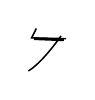
\begin{tikzpicture}[x=0.5cm,y=0.5cm,baseline=0]
\draw[line width=0.55pt] (0.12,0.72)--(0,0.48)--(0.88,0.46);
\draw[line width=1pt] (0.06,0.46)--(0.82,0.43);
\draw[line width=0.55pt] (0.75,0.53) .. controls (0.48,0.16) and (0.18,-0.2) .. (-0.08,-0.36);
\end{tikzpicture}}
\[
(M\longrightarrow\underline{M}(\mathbb{Z}),\quad
\text{and }\underline{M}\xrightarrow{\chi_{\underline{M}}}G_{m\mathbb{Z}}).
\]

Here it will no longer be true in general, I
presume, that the outer homomorphisms \inserted{$\underline{k}_i$} (43)
extend as they stand to homomorphisms
$\underline{T}_i\underset{\unsure{\mathrm{df}}}{=}\underline{T}_{i\mathbb{Z}}\longrightarrow\underline{\Pi}$.
But I \unsure{am going to|have one} consider
the centralizer of $k_i:T_0\longrightarrow\Pi_0$ in $\Pi_0$,
i.e. $\widetilde{L}_{i,0}$ which is a
metabelian group: $\operatorname{Im}(T_0\xrightarrow{k_i}\Pi_0)$ is a
\inserted{normal} subgroup of finite index in it. Consider
the homomorphism
\[
(50)\qquad
\diagram{\begin{tikzcd}[ampersand replacement=\&,column sep=large,row sep=small]
\widetilde{L}_{i,0}\arrow[r]\arrow[d,equal]
\&\underline{\Pi}(\mathbb{Z}),\\
\operatorname{Centr}_{\Pi_0}(k_i:T_0\longrightarrow\Pi_0)\&
\end{tikzcd}}
\]
which is \unsure{entirely} unipotent --- it therefore factors
through a homomorphism of group schemes
\[
(51)\qquad \operatorname{Env}(\widetilde{L}_{i,0})\longrightarrow\underline{\Pi}
\]
(cf.\ \S\,50, $4^\circ$, page\,$658'$ ff), factoring
\margin{212}


\scanpage{214}
through one of the smooth \unsure{quotient|quotients} group \inserted{schemes} \inserted{$\underline{Z}_{i,n}$} of
$\operatorname{Env}(\widetilde{L}_{i,0})$, of which the latter is the $\varprojlim$:
\[
(52)\qquad
\diagram{\begin{tikzcd}[ampersand replacement=\&,column sep=large,row sep=small]
1\arrow[r,no head]\&\underline{nT_0}\arrow[r]
\&\underline{Z}_{i,n}\arrow[r]
\&(H_{i,n})_{S_0}\arrow[r,no head]\arrow[d,phantom,"\simeq"{description,rotate=90}]
\&1\\
\&\&\& (\widetilde{L}_{i,0}/nT_0)\&
\end{tikzcd}}
\]
\margin{$S_0=\operatorname{Spec}\mathbb{Z}$}
But of course, the restriction of the homomorphism
obtained
\[
\unsure{(5|(s}\qquad \underline{Z}_{i,n}\longrightarrow\underline{\Pi}
\]
to
\[
\underline{Z}_{i,n}^{\circ}\simeq\underline{nT_0}
\]
is not in general a monomorphism --- if it
is for fixed $n$, then if $n\mid n'$, $n\ne n'$,
it no longer is for $n'$. A particularly
favorable case would be one where
one can find $n$ such that the induced
homomorphism
\[
(53)\qquad\underline{nT_0}\longrightarrow\underline{\Pi}
\]
\margin{this $n$ is then \uline{unique}.}
is a monomorphism. This implies that the schematic
closure in $\underline{\Pi}$ of the ``$1$-parameter
additive subgroup''
$\deleted{\unsure{\mathcal{G}}}\underline{L}_{i\mathbb{Q}}
=\underline{k}_i(\underline{\unsure{T_0}})$
is a \uline{smooth} subgroup scheme of $\underline{\Pi}$.
\margin{213}

\scanpage{215}
\mspage{755}

This condition should also be sufficient -- at least if one requires that this schematic closure have an identity component which is $\unsure{=|\simeq}$ isomorphic to $\mathrm{G}_{aS_0}$.
We then find, \inserted{in any case,} a unique \uline{monomorphism} (up to conjugation)
\[
(54)\qquad \deleted{\unsure{k}}\uuline{k_i'}:\quad
\diagram{\begin{tikzcd}[ampersand replacement=\&,column sep=large]
\underline{T_0} \arrow[r,hook] \& \underline{\Pi}
\end{tikzcd}}
\]
such that $\uuline{k_i'}_{\mathbb{Q}}$ is of the form $\underline{k_i}_{\mathbb{Q}}\circ(\unsure{r_i}\mathrm{id})$,
\deleted{for}\inserted{with} a suitable $\unsure{\parallel|!!}\ \unsure{r_i}\in\mathbb{Q}^{*+}$.
I am not sure that under these conditions, \deleted{one \unsure{can} find a} \inserted{the }homomorphism deduced from $\underline{k_i'}$ by passing to the $\mathbb{Z}$-points
\[
\diagram{\begin{tikzcd}[ampersand replacement=\&,column sep=large]
T_0\simeq\underline{T_0}(\mathbb{Z}) \arrow[r] \& \underline{\Pi}(\mathbb{Z})
\end{tikzcd}}
\]
factors into a homomorphism
\[
(55)\qquad
\diagram{\begin{tikzcd}[ampersand replacement=\&,column sep=large]
T_0 \arrow[r,"{k_i'\unsure{\varphi|?}}"] \& \Pi_0 \arrow[r,"{\mathrm{can}}"] \& \underline{\Pi}(\mathbb{Z})
\end{tikzcd}},
\]
\unsure{where} $T_0\longrightarrow\Pi_0$ \unsure{belongs} to the \uline{``germ''} $\underline{k_i}$, ---

I will nevertheless take it as an \inserted{additional} hypothesis, when the $\underline{k_i'}$ exist.

I feel like stating a few other ``good hypotheses'', which we will try to \unsure{realize}
\margin{214}

\scanpage{216}

in working on ``integral'' Lie approximations i.e. over $\operatorname{Spec}\mathbb{Z}$.

Consider all possible homomorphisms $\underline{k_i'}$ ($i$ variable, but also by conjugating the original $k_i:\deleted{\unsure{T_0}}\ T_0\longrightarrow\Pi_0$ by arbitrary elements of $\Pi_0$), and the corresponding homomorphisms on the Lie algebras
\[
(56)\qquad \operatorname{Lie}(\underline{k_i'}):\quad
\diagram{\begin{tikzcd}[ampersand replacement=\&,column sep=large,row sep=small]
\deleted{\unsure{\mathbb{Z}}}\ T_0 \arrow[r] \arrow[d,phantom,"{\wr}" description] \& \Gamma\underline{\operatorname{Lie}}(\underline{\Pi})\underset{\unsure{\mathrm{df}}}{=}\operatorname{Lie}(\underline{\Pi}) \\
\begin{gathered}\mathbb{Z}\\\text{(not canonical)}\end{gathered} \&
\end{tikzcd}}
\]
which \unsure{are} by hypothesis \deleted{\unsure{good|a}} universal monomorphisms, we would like $\Gamma\underline{\operatorname{Lie}}(\underline{\Pi})$ to be \uline{generated} (as a $\mathbb{Z}$-module) by their images, or (\unsure{that} which amounts to the same) by the images of a generator of $T_0$.
\margin{this hypothesis \unsure{seems} reasonable in a case like $\Pi_0=\operatorname{SL}(2,\mathbb{Z})$, but \unsure{not if} $I=\varnothing$ for example\ldots !}
\unsure{It|I} amounts to the same to say that if one chooses for $\forall i$ \uline{one} $\underline{k_i'}$, whence the image \inserted{in $\Gamma\underline{\operatorname{Lie}}(\underline{\Pi})$} of a generating element of $T_0$, the $I$ elements obtained in $\deleted{\unsure{\Gamma}}\operatorname{Lie}(\underline{\Pi})$, \uline{and} their conjugates by the elements of $\Pi_0$, generate the $\mathbb{Z}$-module $\operatorname{Lie}(\underline{\Pi})$. This \deleted{means} implies that
\margin{215}

\scanpage{217}
\mspage{756}

this group scheme $\underline{\Pi}^{\circ}$ over $S_0=\operatorname{Spec}\mathbb{Z}$, as an étale sheaf on the ``big étale topos'' of $S_0$, is generated by \deleted{the}\inserted{a finite number of} subgroups $k_i'(\underline{\mathrm{G}_a})$,
\deleted{and by the discrete group $\Pi_0$.}
\inserted{(with possible repetition of the same conjugacy class), or again \deleted{\unsure{rather}}\inserted{that} $\underline{\Pi}$ is}
\deleted{(And there \unsure{arises} \unsure{infinitely|the interesting} \unsure{questi-}}
\inserted{generated by \unsure{the}}
the $k_i'(\mathrm{G}_a)$ (\unsure{their various conjugates|one of each} say) and the discrete group $(\Pi_0)_{S_0}$.
(And there arises the interesting question of making the relations explicit\ldots{} is it enough to write the relations of $\Pi_0$, plus \unsure{the commutativity} of
\[
(57)\qquad
\diagram{\begin{tikzcd}[ampersand replacement=\&,column sep=large,row sep=large]
T_0 \arrow[r,no head,"{k_i'}"] \arrow[d,"{\mathrm{can}}"] \& \Pi_0 \arrow[d,"{\mathrm{can}}"] \\
\underline{T_0} \arrow[r,"{\underline{k_i'}}"] \& \underline{\Pi}
\end{tikzcd}}
\qquad ?\quad\Big)
\]

Other conditions, concerning the group schemes
\[
(58)\qquad
\underline{\gamma}_{\underline{\Pi}}=\underline{\Pi}/\underline{\Pi}^{\circ},\quad
\underline{\gamma}_{\underline{\mathcal{G}}}=\underline{\mathcal{G}}/\underline{\mathcal{G}}^{\circ},\quad
\underline{\gamma}_{\underline{M}}=\underline{M}/\underline{M}^{\circ}
\]
-- we would like these to be \uline{constant} group schemes, \unsure{corresponding} to the \deleted{\unsure{schemes}} finite discrete groups which describe the corresponding quotients of the groups over $\mathbb{Q}$, which discrete groups are quotients
\margin{216}


\scanpage{218}

\[
(59)\qquad
\left\{\begin{array}{l}
\gamma_{\Pi}\ (\text{resp. }\gamma_{\mathcal{G}},\ \text{resp. }\gamma_M)\quad\text{quotients of }\Pi,\mathcal{G},M\\
\underline{\gamma}_{\underline{\Pi}}\simeq(\gamma_{\Pi})_{S_0},\quad
\underline{\gamma}_{\underline{\mathcal{G}}}\simeq(\gamma_{\mathcal{G}})_{S_0},\quad
\underline{\gamma}_{\underline{M}}\simeq(\gamma_M)_{S_0}
\end{array}\right.
\]
which fit into a sequence \deleted{exact}\inserted{of homomorphisms}
\[
(60)\qquad
\diagram{\begin{tikzcd}[ampersand replacement=\&,column sep=large]
\gamma_{\Pi} \arrow[r] \& \gamma_{\mathcal{G}} \arrow[r] \& \gamma_M
\end{tikzcd}}
\]
and into exact sequences
\[
(61)\qquad
\left\{\diagram{\begin{tikzcd}[ampersand replacement=\&,column sep=large,row sep=small]
\gamma_{\Pi} \arrow[r,no head] \& \gamma_{\mathcal{G}} \arrow[r] \& \gamma_{\unsure{\mathcal{T}}} \arrow[r] \& 1\\
\gamma_{\Pi} \arrow[r] \& \gamma_M \arrow[r] \& \gamma_N \arrow[r] \& 1\\
\gamma_{\mathcal{G}} \arrow[r] \& \gamma_M \arrow[r,no head] \& \gamma_{\deleted{\unsure{\mathcal{T}}}\Gamma} \arrow[r] \& 1\\
\gamma_{\unsure{\mathcal{T}}} \arrow[r,no head] \& \gamma_N \arrow[r] \& \gamma_{\Gamma} \arrow[r] \& 1
\end{tikzcd}}\right.\quad .
\]

This hypothesis on $\underline{\Pi},\underline{\mathcal{G}},\underline{M}$ makes it possible to define groups $\underline{\Pi}^{\Delta}(\widehat{\mathbb{Z}})^{\unsure{\Delta}},\underline{\mathcal{G}}^{\Delta}(\widehat{\mathbb{Z}})^{\unsure{\Delta}},\underline{M}^{\Delta}(\widehat{\mathbb{Z}})$, and we shall necessarily have the first two factorizations of
\[
(62)\qquad
\left\{\diagram{\begin{tikzcd}[ampersand replacement=\&,column sep=large,row sep=large]
\Pi \arrow[r] \& \underline{\Pi}^{\Delta}(\deleted{\unsure{\widehat{\mathbb{Q}}}}\widehat{\mathbb{Z}})\\
\mathcal{G} \arrow[r] \& \unsure{\underline{\mathcal{G}}}^{\Delta}(\widehat{\mathbb{Z}})\\
M \arrow[r] \& \underline{M}^{\Delta}(\widehat{\mathbb{Z}})
\end{tikzcd}}\right.
\]
(for
\[
\diagram{\begin{tikzcd}[ampersand replacement=\&,column sep=large,row sep=small]
\Pi_0 \arrow[r,no head] \& \underline{\Pi}(\mathbb{Z})\subset\underline{\Pi}^{\Delta}(\widehat{\mathbb{Z}})\\
\mathcal{G}_0 \arrow[r,no head] \& \underline{\mathcal{G}}(\mathbb{Z})\subset\underline{\mathcal{G}}^{\Delta}(\widehat{\mathbb{Z}})
\end{tikzcd}}
\qquad).
\]
As for the third factorization, it should be included in the starting conditions for a Lie homomorphism of a Teichmüller - Galois structure - namely that $\underline{\unsure{M}}_{\mathbb{Q}}/\underline{\unsure{M}}_{\mathbb{Q}}^{\circ}$ is constant, which makes it possible
\margin{\deleted{\unsure{smooth}}}
\margin{217}


\scanpage{219}
\mspage{757}

then to define $\underline{\unsure{M}}_{\mathbb{Q}}^{\Delta}(\unsure{A|\mathbb{A}}_{\mathbb{Q}})$, and we require that $M\relbar\underline{M}_{\mathbb{Q}}(\unsure{A|\mathbb{A}}_{\mathbb{Q}})$ factor through
\[
(63)\qquad
\diagram{\begin{tikzcd}[ampersand replacement=\&,column sep=large]
M \arrow[r] \& \underline{M}_{\mathbb{Q}}^{\Delta}(\unsure{A|\mathbb{A}}_{\mathbb{Q}})
\end{tikzcd}}\quad .
\]

If moreover we assume that the \unsure{images} of the three homomorphisms (62) are \uline{open} \unsure{subgroups}, (a condition which considerably strengthens the \unsure{index} condition \unsure{given} $4^\circ$) (p. 749), provided we combine it with the surjectivity of the composites
\[
(64)\qquad
\left\{\diagram{\begin{tikzcd}[ampersand replacement=\&,column sep=large,row sep=large]
\Pi \arrow[r,no head] \& \underline{\Pi}^{\Delta}(\widehat{\mathbb{Z}}) \arrow[r] \& \Gamma\underline{\gamma}_{\underline{\Pi}}\\
\mathcal{G} \arrow[r] \& \underline{\mathcal{G}}^{\Delta}(\widehat{\mathbb{Z}}) \arrow[r,no head] \& \Gamma\underline{\gamma}_{\underline{\mathcal{G}}}\\
M \arrow[r,no head] \& \underline{M}^{\Delta}(\widehat{\mathbb{Z}}) \arrow[r,no head] \& \Gamma\underline{\gamma}_{\underline{M}}
\end{tikzcd}}\right.\qquad),
\]
we shall be particularly happy. We shall say that we have a \uline{Lie \deleted{\unsure{homomorphism}}\inserted{approximation}} (over $\mathbb{Z}$, hence ``integral'') \deleted{perfect} non\unsure{degenerate}, if all the additional conditions considered previously are satisfied\ldots
\margin{218}

\scanpage{220}
\uline{Remark} In the preceding presentation, the group $\Pi_0$ \inserted{(or $\unsure{\Pi}$)} itself seems to recede into the background, in favor of $\mathcal{G}_0$ \inserted{(or $\mathcal{G}$)} and its $\mathrm{LT}$-structure. It seems to me indeed that the importance of the role of $\Pi_0$ fades behind that of the \inserted{\unsure{sub-}}group \deleted{\unsure{created|side}} of finite index $\Pi_0'$ (if one exists) which would be \deleted{generated by the $k_i'(T_0)\subset\Pi_0$ (and their} a group with loops and \inserted{of which} the $k_i'(T_0)$ \deleted{\unsure{and}} would be \deleted{conjugates, i.e. $\unsure{\Pi_0''}$, and its \unsure{closure}} exactly the loop subgroups. It is not \inserted{too} clear, even if such a $\Pi_0'$ exists, that it is necessaril\textsuperscript{y} unique (\unsure{let us take|think of} the case for example where $I=\varnothing$ !). The case which had occupied me until now, $\Pi_0=\mathcal{G}_0=\mathcal{G}_{0,3}^{+}\unsure{=|\text{--}}\unsure{\mathcal{G}_{1,1}^{+}|\mathcal{T}_{1,1}^{+}}$, has been a little ``misleading'', for \unsure{we then took} $\Pi_0:=\mathcal{G}_0$ \deleted{\unsure{this}} \unsure{precisely}. If we had thought \deleted{\unsure{As we}} \inserted{\unsure{in desire}} \unsure{right} at the beginning of \unsure{my work}, where \inserted{\unsure{by taking only}} $\Pi_0=\Pi_{0,3}$ as the starting group, we would have seen (as was moreover actually the case) the role of $\Pi_{0,3}$ dwindle in favor of the smaller subgroups (type $\Pi^{\unsure{\sharp}}$, giving rise to the $\mathcal{G}^{\unsure{\leftrightarrow}}$ of \S\,49 $\overline{\underline{\mathrm{VI}}}$\ldots)
\margin{219}

\scanpage{221}
\mspage{758}
$4^\circ)$ \uline{Lie} \deleted{\uline{hom}}\inserted{approximation} \inserted{of $(\Pi_0,\mathcal{G}_0,M)$} \uline{induced by an approximation of} $\mathcal{G}_0$.

Let us start with a system $(\mathcal{G}_0\supset\Pi_0)$ of a \inserted{discrete} $\mathrm{LT}$-group $\mathcal{G}_0$, and of an invariant \inserted{$L$-}subgroup $\Pi_0$ of $\mathcal{G}_0$. Suppose \unsure{given} group \unsure{scheme} $\underline{\mathcal{G}}_{\mathbb Q}$ over $\mathbb Q$, and a homomorphism
\margin{We assume that the homomorphism $\unsure{\mathcal{G}_0}\longrightarrow\mathbb Z^*=\{\pm1\}$ defined by the action of $\mathcal{G}_0$ on the $L$-group $\Pi_0$ (\unsure{multipliers}) is trivial\ldots}
\diagram{\begin{tikzcd}[ampersand replacement=\&,column sep=large]
(65)\quad\varphi:\ \mathcal{G}_0 \arrow[r] \& \underline{\mathcal{G}}(\mathbb Q)
\end{tikzcd}}
having the property that for $\forall$ homomorphism
\diagram{\begin{tikzcd}[ampersand replacement=\&,column sep=large]
(66)\quad k_i:\ T_0 \arrow[r] \& \mathcal{G}_0
\end{tikzcd}}
which \unsure{is} part of the $\mathrm{LT}$-structure, the composite homomorphism
\diagram{\begin{tikzcd}[ampersand replacement=\&,column sep=large]
T_0 \arrow[r] \& \mathcal{G}_0 \arrow[r,no head] \& \underline{\mathcal{G}}(\mathbb Q)
\end{tikzcd}}
is quasi-unipotent. We assume moreover that $\underline{\mathcal{G}}_{\mathbb Q}$ is \uline{generated} by the set of \deleted{\unsure{its}} $\mathbb Q$-rational points \unsure{defined} by the elements of $\mathcal{G}_0$ via (65).

We consider $\underline{\mathcal{G}}_{\mathbb Q}$ as equipped with the homomorphism (65) and with the family of outer homomorphisms
\diagram{\begin{tikzcd}[ampersand replacement=\&,column sep=large]
(67)\quad\underline{k}_i:\ \underline{T_0}_{\mathbb Q} \arrow[r] \& \underline{\mathcal{G}}_{\mathbb Q}
\end{tikzcd}}
\margin{220}

\scanpage{222}
giving rise to compatibilities
\diagram{\begin{tikzcd}[ampersand replacement=\&,column sep=huge,row sep=large]
T_0 \arrow[r,"k_i"] \arrow[d,"\mathrm{can}"',"{\deleted{\unsure{\varphi}}}"] \& \mathcal{G}_0 \arrow[d,"{(65)}"] \\
(68)\quad\underline{T_0}_{\mathbb Q}(\mathbb Q) \arrow[r,"\underline{k}_i(\mathbb Q)"] \arrow[r,shorten >=12pt] \& \underline{\mathcal{G}}(\mathbb Q).
\end{tikzcd}}

I then consider the group scheme over $\mathbb Q$ of \inserted{\deleted{pairs} pairs $(u,\mu)$ of an} \unsure{automorphisms|automorphism} of $\underline{\mathcal{G}}_{\mathbb Q}$, and of a $\mu\in\Gamma G_{\mathrm m}$, \unsure{such|such} that for $\forall\ i\in I$, \deleted{we have} there exists locally a section $f_i$ of $\underline{\Pi}_{\mathbb Q}$ (generated by the image of $\Pi_0$ in $\underline{\mathcal{G}}(\mathbb Q)$), \unsure{such|such} that we have
\[
(69)\qquad u\bigl(\underline{k}'_i(\lambda)\bigr)=\operatorname{int}(f_i)^{-1}(\mu\lambda).
\]
I denote by $\underline{M}_{\mathbb Q}^{\varphi}$ this group scheme over $\mathbb Q$, augmented to $G_{\mathrm m\mathbb Q}$ by $(u,\mu)\longmapsto\mu$, by a homomorphism which is trivial on $\operatorname{Im}(\underline{\mathcal{G}}_{\mathbb Q}\to\underline{M}_{\mathbb Q}^{\varphi})$, hence factors through a homomorphism
\diagram{\begin{tikzcd}[ampersand replacement=\&,column sep=large]
(70)\quad\underline{\Gamma}_{\mathbb Q}^{\varphi}\overset{\mathrm{déf}}{=}\underline{M}_{\mathbb Q}^{\varphi}/\operatorname{Im}\underline{\mathcal{G}}_{\mathbb Q} \arrow[r,"\chi_{\underline{\Gamma}}"] \& G_{\mathrm m\mathbb Q}.
\end{tikzcd}}
If now $(\mathcal{G}_0,\Pi_0)$ is part of a Galois-Teichmüller system
\margin{221}

\scanpage{223}
\mspage{759}
\diagram{\begin{tikzcd}[ampersand replacement=\&,column sep=small,row sep=small]
(\Pi \arrow[r,phantom,"\subset" description] \& \mathcal{G} \arrow[r,phantom,"\subset" description] \& M), \\
\Pi_0 \arrow[u,phantom,"\cup" description] \arrow[r,phantom,"\subset" description] \& \mathcal{G}_0 \arrow[u,phantom,"\cup" description] \& {}
\end{tikzcd}}
and \uline{if} $\mathcal{G}_0\xrightarrow{\varphi}\underline{\mathcal{G}}_{\mathbb Q}^{\deleted{\unsure{\varphi}}}$ comes from a Lie homomorphism of this system, $M\longrightarrow\underline{M}(\unsure{A|\mathbb{A}}_{\mathbb Q})$, by the method of the preceding section, then we find a \unsure{natural} homomorphism
\diagram{\begin{tikzcd}[ampersand replacement=\&,column sep=large]
(71)\quad\underline{M}_{\mathbb Q} \arrow[r] \& \underline{M}_{\mathbb Q}^{\varphi},
\end{tikzcd}}
\margin{via the operation of $\underline{M}_{\mathbb Q}$ on $\underline{\mathcal{G}}_{\mathbb Q}$, and $\chi_{\underline{M}}$}
making the diagram commutative
\diagram{\begin{tikzcd}[ampersand replacement=\&,column sep=large,row sep=large,/tikz/execute at end picture={
\begin{scope}[overlay]
\draw ([xshift=-4mm,yshift=-3mm]\tikzcdmatrixname-1-1.south west) -- ([xshift=4mm,yshift=5mm]\tikzcdmatrixname-1-1.north east);
\draw ([xshift=-5mm,yshift=-1mm]\tikzcdmatrixname-2-1.north west) -- ([xshift=1mm,yshift=2mm]\tikzcdmatrixname-1-2.north west);
\draw ([xshift=-3mm,yshift=-1mm]\tikzcdmatrixname-2-1.south west) -- ([xshift=6mm,yshift=0mm]\tikzcdmatrixname-1-2.south east);
\draw ([xshift=-3mm,yshift=-2mm]\tikzcdmatrixname-3-1.south west) -- ([xshift=7mm,yshift=1mm]\tikzcdmatrixname-2-2.south east);
\draw ([xshift=0mm,yshift=-4mm]\tikzcdmatrixname-3-1.south east) -- ([xshift=5mm,yshift=2mm]\tikzcdmatrixname-3-2.north east);
\end{scope}
}]
\deleted{\mathcal{G}_0} \arrow[r] \arrow[d] \& \deleted{M} \arrow[d] \& {} \& \underline{\mathcal{G}}_{\mathbb Q} \arrow[r] \arrow[dr,"\mathrm{can.}","{\begin{gathered}\text{via \unsure{automorphisms}}\\\mathrm{int.}\end{gathered}}"'] \& \underline{M}_{\mathbb Q} \arrow[d] \\
(72)\quad\deleted{\underline{\mathcal{G}}(\mathbb Q)} \arrow[r,no head] \arrow[d,"{\deleted{\underline{\mathrm{int}}}}"'] \arrow[dr] \& \deleted{\underline{M}(\unsure{A|\mathbb{A}}_{\mathbb Q})} \arrow[d] \& {} \& {} \& \underline{M}_{\mathbb Q}^{\varphi}. \\
\deleted{\underline{M}_{\mathbb Q}^{\varphi}(\mathbb Q)} \arrow[r,hook] \& \deleted{\underline{M}_{\mathbb Q}^{\varphi}(\unsure{A|\mathbb{A}}_{\mathbb Q})} \& {} \& {} \& {}
\end{tikzcd}}

If the center of $\underline{\mathcal{G}}_{\mathbb Q}$ is trivial (which is a ``credible'' hypothesis especially if the center of $\mathcal{G}_0$ is so\ldots) then $\underline{\mathcal{G}}_{\mathbb Q}\longrightarrow\underline{M}_{\mathbb Q}^{\varphi}$ is injective, and $\underline{\mathcal{G}}_{\mathbb Q}$ is interpreted as ``the $\underline{\mathcal{G}}_{\mathbb Q}$'' associated to a Lie homomorphism
\diagram{\begin{tikzcd}[ampersand replacement=\&,column sep=large]
{\left(\begin{array}{ccccc}
\unsure{\pi|\Pi}&\subset&\mathcal{G}&\subset&M\\[-1pt]
\cup&&\cup&&\\[-1pt]
\Pi_0&\subset&\mathcal{G}_0&&
\end{array}\right)} \arrow[r] \& (\underline{\Pi}\subset\underline{\mathcal{G}}_{\mathbb Q}\subset\underline{M}_{\mathbb Q}^{\varphi}),
\end{tikzcd}}
which has a certain universal character with respect to the given homomorphism (65) $\varphi:\mathcal{G}_0\longrightarrow\underline{\mathcal{G}}(\mathbb Q)$.
\margin{222}

\scanpage{224}
When we do not assume in advance the existence of a \deleted{$\unsure{M|H}$} Lie homomorphism in which $\underline{\mathcal{G}}_{\mathbb Q}$ fits, it is not automatic that we can find a homomorphism
\diagram{\begin{tikzcd}[ampersand replacement=\&,column sep=large]
(73)\quad\varphi_M:\ M \arrow[r] \& \underline{M}_{\mathbb Q}^{\varphi}(\unsure{A|\mathbb{A}}_{\mathbb Q})
\end{tikzcd}}
which accounts for the operations of $M$ on $\mathcal{G}_{\deleted{\unsure{0|\mathbb Q}}}$, through the commutativity of a diagram, for $\forall\ g\in M$
\diagram{\begin{tikzcd}[ampersand replacement=\&,column sep=large,row sep=large,/tikz/execute at end picture={
\begin{scope}[overlay]
\draw ([xshift=-1mm,yshift=-1mm]\tikzcdmatrixname-1-1.east) -- ([xshift=-8mm,yshift=-2mm]\tikzcdmatrixname-1-2.west);
\end{scope}
}]
\deleted{M} \arrow[r] \& \mathcal{G} \arrow[r,"{\operatorname{int}(g)|\mathcal{G}}"] \arrow[r,shorten >=12pt] \arrow[d,"\widehat{\varphi}"'] \& \mathcal{G} \arrow[d,"\widehat{\varphi}"] \\
(74) \& \underline{\mathcal{G}}(\unsure{A|\mathbb{A}}_{\mathbb Q}) \arrow[r,"{\operatorname{int}(\varphi_M(g))|\underline{\mathcal{G}}(\unsure{A|\mathbb{A}}_{\mathbb Q})}"'] \& \underline{\mathcal{G}}(\unsure{A|\mathbb{A}}_{\mathbb Q}).
\end{tikzcd}}

We are mainly interested in those $\varphi$ (65) for which (73) exists --- at least after possibly restricting to an open \unsure{subgroup|subgroup} of $M$\ldots
\margin{223}

\scanpage{225}
\mspage{760}

\uline{53}

$1^\circ)$ \unsure{Differentiable|Differential} action and special Teichmüller group.

Let $X$ be a connected \inserted{\deleted{\unsure{compact}} differentiable,} orientable surface (compact in the case of interest to us), $I$ a discrete subset of $X$. For $\forall i\in I$, let $\mathbb{S}_i$ be the space (homeomorphic to the \deleted{\unsure{c|d}} \unsure{circle}) of homogeneous half-lines in the tangent space, and let $\widetilde{\mathbb{S}}_i$ be a universal covering of $\mathbb{S}_i$.

Let \deleted{\unsure{Let} $\unsure{\widetilde g}$} $\unsure{u}$ be a differentiable automorphism of $(X,S)$, it induces an automorphism of
\[
(1)\qquad \mathbb{S}=\mathbb{S}_I\overset{\mathrm{d\acute ef}}{=}\coprod_{i\in I}\mathbb{S}_i,
\]
denoted $u_{\mathbb{S}}$. Let us consider the set of liftings \inserted{$\widetilde u$} of $u_{\mathbb{S}}$ to an automorphism of \deleted{$\unsure{\mathbb{S}}$ of $\unsure{\widetilde{\mathbb{S}}}$}
\[
(2)\qquad \widetilde{\mathbb{S}}=\coprod_{i\in I}\widetilde{\mathbb{S}}_i.
\]
Let us note, if $T_0$ is the orientation module of $X$, that \deleted{each} $T_0$ operates on each $\widetilde{\mathbb{S}}_i$,

\margin{224}

\scanpage{226}

so that $T_0$ in fact operates on $\mathbb{S}$ and
\[
(3)\qquad \widetilde{\mathbb{S}}/T_0\simeq\mathbb{S}.
\]
This shows that (if $u$ is as above) the group $T_0^I$ operates on the left (for example) on the set of liftings $\widetilde u$\unsure{.} which thus becomes a torsor under $T_0^I$.

Let $G$ be a topological group, which operates \unsure{differentiably} on $(X,S)$, with \deleted{\unsure{of|some}} \unsure{one} \inserted{\unsure{of the}} continuous actions on $\mathbb{S}$. We set
\[
(4)\qquad \widetilde G=
\left\{(\deleted{\unsure{g}}\unsure{u},\widetilde u)\;\middle|\;
\begin{array}{l}
u\in G,\quad\widetilde u\text{ a continuous lifting}\\
\text{of }u_{\mathbb{S}}\text{ to }\widetilde{\mathbb{S}}
\end{array}
\right\},
\]
we find on $\widetilde G$ a canonical topology \inserted{(convergence of $u$ and uniform convergence of $\widetilde u$)}, which is such that the homomorphism $G\longrightarrow\widetilde G$ \unsure{makes|will make} $G$ a covering of $\widetilde G$, with group $\unsure{T}_0^I$:
\[
(6)\qquad
\diagram{\begin{tikzcd}[ampersand replacement=\&,column sep=large]
1\arrow[r,no head] \& T_0^I\arrow[r] \& \widetilde G\arrow[r] \& G\arrow[r] \& 1
\end{tikzcd}}.
\]
\margin{\uline{N.B.} $G$ operates on $T_0^I$ via the character \deleted{$\unsure{(52)|(\varepsilon)}$} of orientation}

\uline{Proposition} \deleted{\unsure{If}} Suppose that $X$ is \unsure{compact|compact},

\margin{225}

\scanpage{227}
\mspage{761}

and consider the canonical homomorphism
\[
\diagram{\begin{tikzcd}[ampersand replacement=\&,column sep=large]
G\arrow[r] \& G/G^\circ\arrow[r] \& \mathcal{T}(X,S)
\end{tikzcd}}
\]
(Teichmüller group \inserted{of $(X,S)$}), we then have a canonical homomorphism of extensions
\[
(7)\qquad
\diagram{\begin{tikzcd}[ampersand replacement=\&,column sep=large,row sep=large]
1\arrow[r,no head] \& T_0^I\arrow[r]\arrow[d,"1"] \& \widetilde G\arrow[r]\arrow[d] \& G\arrow[r,no head]\arrow[d] \& 1\\
1\arrow[r] \& T_0^I\arrow[r] \& \mathrm{Sp}\mathcal{T}(X,S)\arrow[r] \& \mathcal{T}(X,S)\arrow[r,no head] \& 1
\end{tikzcd}},
\]
$\mathrm{Sp}\mathcal{T}(X,S)$ is the \uline{special} Teichmüller group of $(X,S)$.

\margin{For the proof cf. the developments of $5^\circ)$ (pages $766'$ ff, \unsure{in particular} pages \unsure{784} ff)}

\uline{N.B.} We shall note that if for $\forall i$ \inserted{$\in I$}, we fix an origin $e_i$ on $\mathbb{S}_i$, then it follows from the universal property of $\widetilde{\mathbb{S}}$ that giving a lifting $\widetilde u$ of $u_{\mathbb{S}}$ to $\widetilde{\mathbb{S}}$ amounts to giving, for $\forall i\in I$, a lifting of $u_{\mathbb{S}}(e_i)$ to a point $\widetilde a_i$ of $\widetilde{\mathbb{S}}_{\unsure{u(e_i)|u(i)}}$ (i.e., of $\widetilde{\mathbb{S}}_{u(i)}$).

\margin{226}

\scanpage{228}

$2^\circ)$ \uline{The groups} $\mathrm{GL}(2,\mathbb{R})^{\pm1}$\unsure{${}^{\sim}$|and} \deleted{$\unsure{\mathrm{GL}(2,\mathbb{Z})}$}. \inserted{We set}
\[
(8)\qquad \mathrm{GL}(2,\mathbb{R})^{\pm1}
=\{u\in\mathrm{GL}(2,\mathbb{R})\mid\det u\in\{\pm1\}\}.
\]
This group operates \unsure{differentiably} on $\mathbb{C}\simeq\mathbb{R}^2$ leaving the origin fixed, we can therefore apply the construction \unsure{of} $1^\circ)$, Here $\mathbb{S}_0$ is identified with the unit circle
\[
(9)\qquad
\diagram{\begin{tikzcd}[ampersand replacement=\&,column sep=large]
\mathbb{U}\overset{\mathrm{d\acute ef}}{=}\{z\in\mathbb{C}\mid|z|=1\}\arrow[r] \& \mathbb{S}_0^{\unsure{\deleted{*}|*}}\\
z\arrow[r,mapsto] \& \mathbb{R}^{+}z
\end{tikzcd}}
\]
and for $u\in\mathrm{GL}(2,\mathbb{R})^{\unsure{\pm1}}$, its action on $\mathbb{S}_0^{\unsure{\deleted{*}|*}}$ is identified with the action on $\mathbb{U}$ given by
\[
(10)\qquad
\diagram{\begin{tikzcd}[ampersand replacement=\&,column sep=large,row sep=0.3em]
z\arrow[r,mapsto] \& \dfrac{u(z)}{|z|}\\
\mathbb{U}\arrow[u,phantom,"\in"{rotate=90}]
\end{tikzcd}}.
\]
A lifting of this action \inserted{$u_{\mathbb{S}_0^{\unsure{\deleted{*}|*}}}$} to an action on $\widetilde{\mathbb{S}}_0^{\unsure{\deleted{*}|*}}$ amounts to a lifting of $u(\unsure{e_0}=1)$ to an element of $\widetilde{\mathbb{S}}_0$. \deleted{\unsure{and}}
We \deleted{\unsure{shall choose|shall describe} the covering} \inserted{\unsure{shall construct|construct} $\widetilde{\mathbb{S}}$ \deleted{$\unsure{\widetilde{\mathbb{S}}_0}$}} by choosing a base point $e_0$ of $\mathbb{S}_0$, corresponding to the

\margin{227}
